\documentclass[12pt,a4paper]{report}
\usepackage[utf8]{inputenc}
\usepackage[english]{babel}
\usepackage{amsmath}
\usepackage{amsfonts}
\usepackage{amssymb}
\usepackage{graphicx}
\usepackage{cite}
\usepackage[left=2cm,right=2cm,top=2cm,bottom=2cm]{geometry}
\author{Josep Puig Ruiz}
\title{Communication Power Required and Transmission Time}
\begin{document}
\maketitle
\chapter{Communication Power Required and Transmission Time}
\section{Types of Global Satellite Systems}
The evolution from geo-stationary to low-Earthorbit (LEO) satellites has resulted in a number of proposed global satellite systems, which can be grouped into three distinct types - Little LEOs, Big LEOs, and Broadband LEOs. 
In the following table we can see the man applications of the different global satellite systems.\\
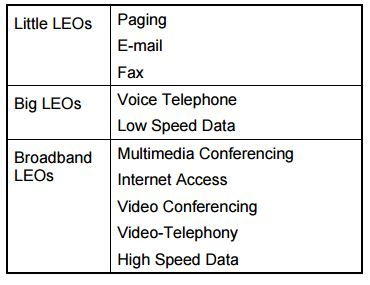
\includegraphics[scale=1]{Types.jpg}  \\
Therefore, the network that Astrea aims to provide would belong to broadband LEOs satellite systems. 
\section{Broadband LEOs}
It can be taken as example the Teledesic system (from late nineties). It did not intend to market services directly to end-users, but to provide an open network for delivery of such services by others. This is kind of similar to what Astrea intends to do. Therefore, it is a good example and some figures from it can be taken and analyzed. \\
Teledesic used small, "earth-fixed" cells both for efficient spectrum utilization and to respect country's territorial boundaries. Within a 53km x 53km, the Network was able to accomodate over 1800 simultaneous 16 Kbps voice channels. Channel bandwiths are assigned dynamically and assymetrically, and range from 16 Kbps to 2 Mbps (uplink), and up to 28 Mbps on the downlink. \\
This network was orginised as follows: 21 circular orbit planes, which were staggered in altitude between 695 and 705 km. Each plane used to contain a minimum of 40 operational satellites plus up to four on-orbit spares spaced evenly around the orbit, for a total of 924 satellites. Those planes were at a sun-syncronous inclination (approx. 98.16º), i.e, constant angle relative to the sun. \\


Webs (sé que falta poner la bibliografía bien, es para no perder los enlaces, pendiente). \\
goo.gl/pUqga9 \\
http://ntrs.nasa.gov/archive/nasa/casi.ntrs.nasa.gov/19960054092.pdf \\
http://www.satsig.net/latency.htm \\


\section{Latency}
Latency in satellite communications is the time that the radio signal (wave) takes to travel to and from the satellite in the space. \\
Example of how to calculate the latency of an orbit 1500 km above Earth:\\
1500km *1000m/km / 3*10^8 (speed of light) = .005s * 4s/trip = .02 seconds = 20 ms \\

More data about the designed satellite and power of antennas and so is required to take a study any further. \\
\bibliographystyle{plain}
\bibliography{library}
\end{document}